% Source: https://github.com/Oriolac/tfg

% !TeX spellcheck = ca
\documentclass[11pt, a4paper]{article}

\setcounter{secnumdepth}{5}
\setcounter{tocdepth}{5}
\newcommand\simpleparagraph[1]{%
  \stepcounter{paragraph}\paragraph*{\theparagraph\quad{}#1}}

\usepackage[utf8]{inputenc}

\usepackage{latexsym}
\usepackage{float}
\usepackage[utf8]{inputenc}
%\usepackage[catalan]{babel}
\usepackage[english]{babel}
\usepackage{microtype}
\usepackage[hyphens]{url}
\usepackage[hyperfootnotes=false]{hyperref}
\usepackage{graphicx}
\usepackage{makeidx}
\usepackage{datetime}
\usepackage{multicol}
\usepackage{setspace}
\usepackage{enumerate}
\usepackage{booktabs}
\usepackage{braket}
\usepackage{listings}
\usepackage{color}
\usepackage{amsmath}
\usepackage{amssymb}
\usepackage[table,xcdraw]{xcolor}
\usepackage{graphicx}
\usepackage{listings}
\usepackage{hyperref}
\usepackage{vmargin}
\usepackage{wrapfig}
\usepackage{subfiles}
\usepackage{float}
\usepackage{amsmath}
\usepackage{amssymb}
\usepackage{tikz-cd}
\usepackage{multirow}
\usepackage{pgffor}
\usepackage{enumitem}
\usepackage{iflang}
\usepackage{varioref}
\usepackage{hyperref}
\usepackage{cleveref}
\usepackage{caption}
\usepackage{subcaption}
\usepackage{tikz}
\usepackage{enumitem}
\usepackage{xpatch}
\usepackage{refcount}
\usepackage{color}
\usepackage{pdfpages}
\usepackage[stable]{footmisc}


%%%%%%%%%%%%%%%%%%%%%%%%%%%%%%%%%%%%%%%
%%%%%%%%%%%% UTIL COMMANDS %%%%%%%%%%%%  

\setcounter{secnumdepth}{4}
\newcommand{\nc}{\newcommand}
\nc{\supindex}{\textsuperscript}
\renewcommand{\baselinestretch}{1.5}
\nc{\myparagraph}[1]{\paragraph{#1}\mbox{}\\}

%%%%%%%%%%%%%%%%%%%%%%%%%%%%%%%%%%%%%%%
%%%%%%%%%%%%% CONFIG FILE %%%%%%%%%%%%%

\nc{\mytitle}{Glaucoma Detection with Retinal Fundus Images using Machine Learning}
\nc{\mysubtitle}{Bayesian Inference}
\nc{\authors}{Àiax Faura Vilalta}
\nc{\datetime}{30\supindex{th} of June, 2022}
\nc{\assignatura}{Treball Final de Grau}
\nc{\professorat}{Jordi Planes Cid, Josep Argelich Romà}

% Per separar professors, utilitzar ','
% 	Ex: Maria, Joan, Pere

%%%%%%%%%%%%%%%%%%%%%%%%%%%%%%%%%%%%%%%
%%%%%%%%%%%%%  LANGUAGE   %%%%%%%%%%%%%

\newcommand{\tr}{\IfLanguageName{english}}

%%%%%%%%%%%%%%%%%%%%%%%%%%%%%%%%%%%%%%%
%%%%%%%%%%%%%%%%% MATH %%%%%%%%%%%%%%%%

\nc{\prob}[1]{P({#1})}
\nc{\probl}[2]{P({#1}|{#2})}

%%%%%%%%%%%%%%%%%%%%%%%%%%%%%%%%%%%%%%%
%%%%%%%%%%%%% FUNCTIONS %%%%%%%%%%%%

\nc{\numitems}[1]{\getrefnumber{#1}}
\newcounter{itemcntr}
\AtBeginEnvironment{itemize}{%
	\setcounter{itemcntr}{0}%
	\xapptocmd{\item}{\refstepcounter{itemcntr}}{}{}%
}

\setpapersize{A4}

\author{Àiax Faura Vilalta}
\date{30th of June, 2022}

\def\contentsname{Contents}
\begin{document}

\definecolor{gray}{rgb}{0.4,0.4,0.4}
\definecolor{darkblue}{rgb}{0.0,0.0,0.6}
\definecolor{cyan}{rgb}{0.0,0.6,0.6}
\lstset{
	basicstyle=\ttfamily,
	columns=fullflexible,
	showstringspaces=false,
	commentstyle=\color{gray}\upshape
}

\lstdefinelanguage{XML}
{
	morestring=[b]",
	morestring=[s]{>}{<},
	morecomment=[s]{<?}{?>},
	stringstyle=\color{black},
	identifierstyle=\color{darkblue},
	keywordstyle=\color{cyan},
	morekeywords={xmlns,version,type}% list your attributes here
}


% \begin{titlepage}
% \begin{figure}[htb]
% \begin{center}
% 	
\includegraphics[width=5cm]{imgs/UDL.png}
%   	\vspace*{\stretch{1.0}}
%   	\\
%   	\medskip
%   	\begin{center}
%   		\medskip\bigskip\bigskip\bigskip
  		
%      	\huge\textbf{\mytitle}
%      	\\\medskip 	\Large  
     	
     	
%      	\bigskip\bigskip\bigskip
%      	\bigskip
%      	\normalsize{\tr{Made by}{Made by:}}
%      	\\
%      	\large\textit{\authors}
%      	\\
%      	\setlength{\parskip}{1em}
%      	\normalsize{\tr{Delivery}{Delivery:}}
%      	\\
%      	\large{\datetime}
%      	\end{center}
%   	\vspace*{\stretch{2.0}}
% \end{center}
% \end{figure}
% \begin{flushright}
% Universitat de Lleida
% \\
% Escola Politècnica Superior
% \\
% Grau en Enginyeria Informàtica
% \\
% \assignatura
% \\
% \medskip
% \textbf{\tr{Professorate:}{Tutor:}}
% \\
% \foreach \n in \professorat{\n\\}
% \end{flushright}
% \thispagestyle{empty} 
% \end{titlepage}
\tableofcontents
\thispagestyle{empty} 
\newpage
\listoffigures
\listoftables
\thispagestyle{empty}
\newpage
\section*{Acknowledgments}
I want to thank my family and friends for being a great support throughout this experience. To the tutors of this bachelor thesis with a special mention to Jordi for the idea of this project. Their guidance and recommendations helped make this project more interesting and taught me valuable lessons. Finally, I would also like to thank Mariano Garralda for his advices on some aspects of the project.
\newpage
\section*{Abstract}
Glaucoma is a group of eye diseases that affects around 80 million people worldwide and can lead to major problems such as blindness if not treated early. The goal of this project is to automate glaucoma detection so that more people can be treated before the disease causes irreversible damage. To do this, different machine learning techniques have been studied and implemented to detect glaucoma with retinal fundus images. After evaluating all the models developed with the aim of achieving the automation of glaucoma detection, the best score went to VGG16 with transfer learning, more specifically, feature extraction. Other techniques have been used to train the model, such as balanced data augmentation to deal with the small biased dataset. Furthermore, the predictions of this model have been interpreted with the lime framework to see if the model is trustable or if it only works well by coincidence. In the end, the model scores for the defined evaluation have not reached the high standards expected for a problem involving people's health. And interpretations of the predictions have shown that the model was not focusing on the important parts of the retinal fundus images. However, a possible future work that could improve this project results has been proposed. Although the results were not the desired ones, the project offers useful resources to inquire more into this project or other similar projects of binary classification of images.

\newpage
\section{Introduction}
Glaucoma is a group of eye diseases that can cause vision loss and blindness by damaging a nerve in the back of the eye called the optic nerve, see Figure \ref{fig:Glaucoma_explanation_visualized}. It affects around 80 million people worldwide and its a growing problem as each year there are more cases. This is because life expectancy is increasing and one of the main groups affected by this disease is people over 60 years of age. Other people prone to this disease are African-American people over 40 years of age, relatives of people already diagnosed with glaucoma, diabetics, steroid users, among others.
\begin{figure}[H]
	\centering
	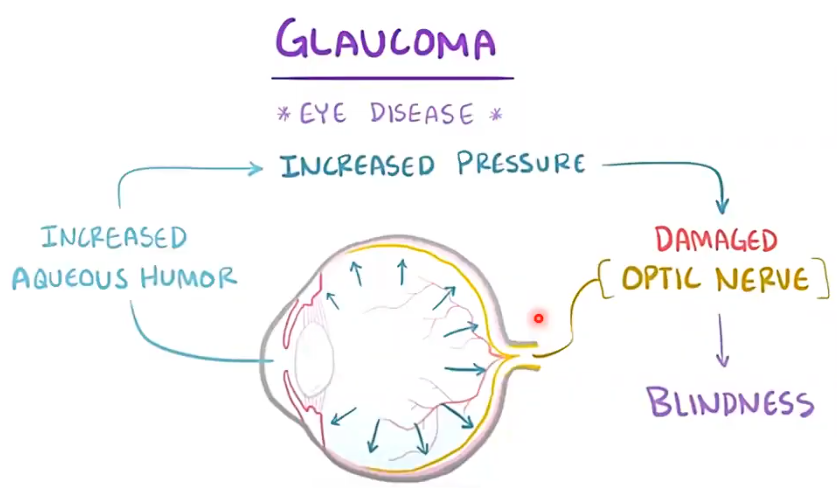
\includegraphics[width=14cm]{imgs/general/Glaucoma_explanation_visualized.PNG}
	\caption{Visual explanation of glaucoma}
	 \label{fig:Glaucoma_explanation_visualized}
\end{figure}
\noindent Glaucoma can be treated to prevent further problems, either with medication, laser treatment, or surgery. These treatments can prevent patients' vision from getting worse, but they don't undo any damage already done. This is why it is so important to get treatment as soon as possible. However, glaucoma screening can involve a few different and recurring tests, which leads to the main problem: there are not enough experts to perform early detection in a large population. That is why automating this process could help treat more people and preserve a good quality of life for those affected by this problem.
\\
\\
One possible approach to automate glaucoma detection could be the use of artificial intelligence. Artificial intelligence (AI) is a wide-ranging branch of computer science concerned with building smart machines capable of performing tasks that normally require human intelligence. AI has been successfully used in many different fields, including medicine, where it helped solve problems and in some cases performed even better than humans.
Nevertheless, in the field of medicine, AI is often used to help humans by giving them knowledge that they cannot perceive or that can save them time. The latter could be useful in this case because, although the ideal would be to have an artificial intelligence that could detect glaucoma on its own with 100\% reliability, this is not always the case. Therefore, saving clinicians time in their diagnosis by suggesting which people are more at risk of glaucoma is also a good approach that will be studied in this document.
\\
\\
One way to replicate human behavior to detect glaucoma without being an expert could be to have a machine learn by giving it some examples of what glaucoma is or is not. The branch of AI that studies how to do this is Machine Learning, which focuses on using data and algorithms to mimic the way humans learn, gradually improving their accuracy. The data that the algorithms will use to detect glaucoma is the same data that optometrists use in one of the glaucoma detection tests they perform, the retinal fundus images. Retinal fundus images show the inner surface of the eye, including the retina, retinal vasculature, optic disc, macula, and posterior pole. See Figure \ref{fig:Retinal_fundus_image_obtention} and \ref{fig:Retinal_fundus_image}. Experts use different methods to detect glaucoma with these images, which will be explained later in the ``Problem Analyisis" section.
\begin{figure}[H]
\centering
\begin{minipage}{.5\textwidth}
  \centering
  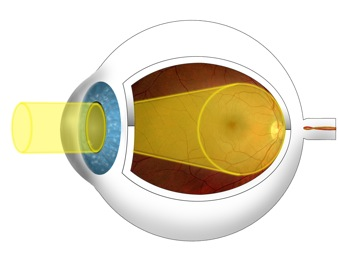
\includegraphics[width=7cm, height=6cm]{imgs/general/Retinal_fundus_image_obtention.jpg}
  \captionof{figure}{Retinal fundus image obtention}
  \label{fig:Retinal_fundus_image_obtention}
\end{minipage}%
\begin{minipage}{.5\textwidth}
  \centering
  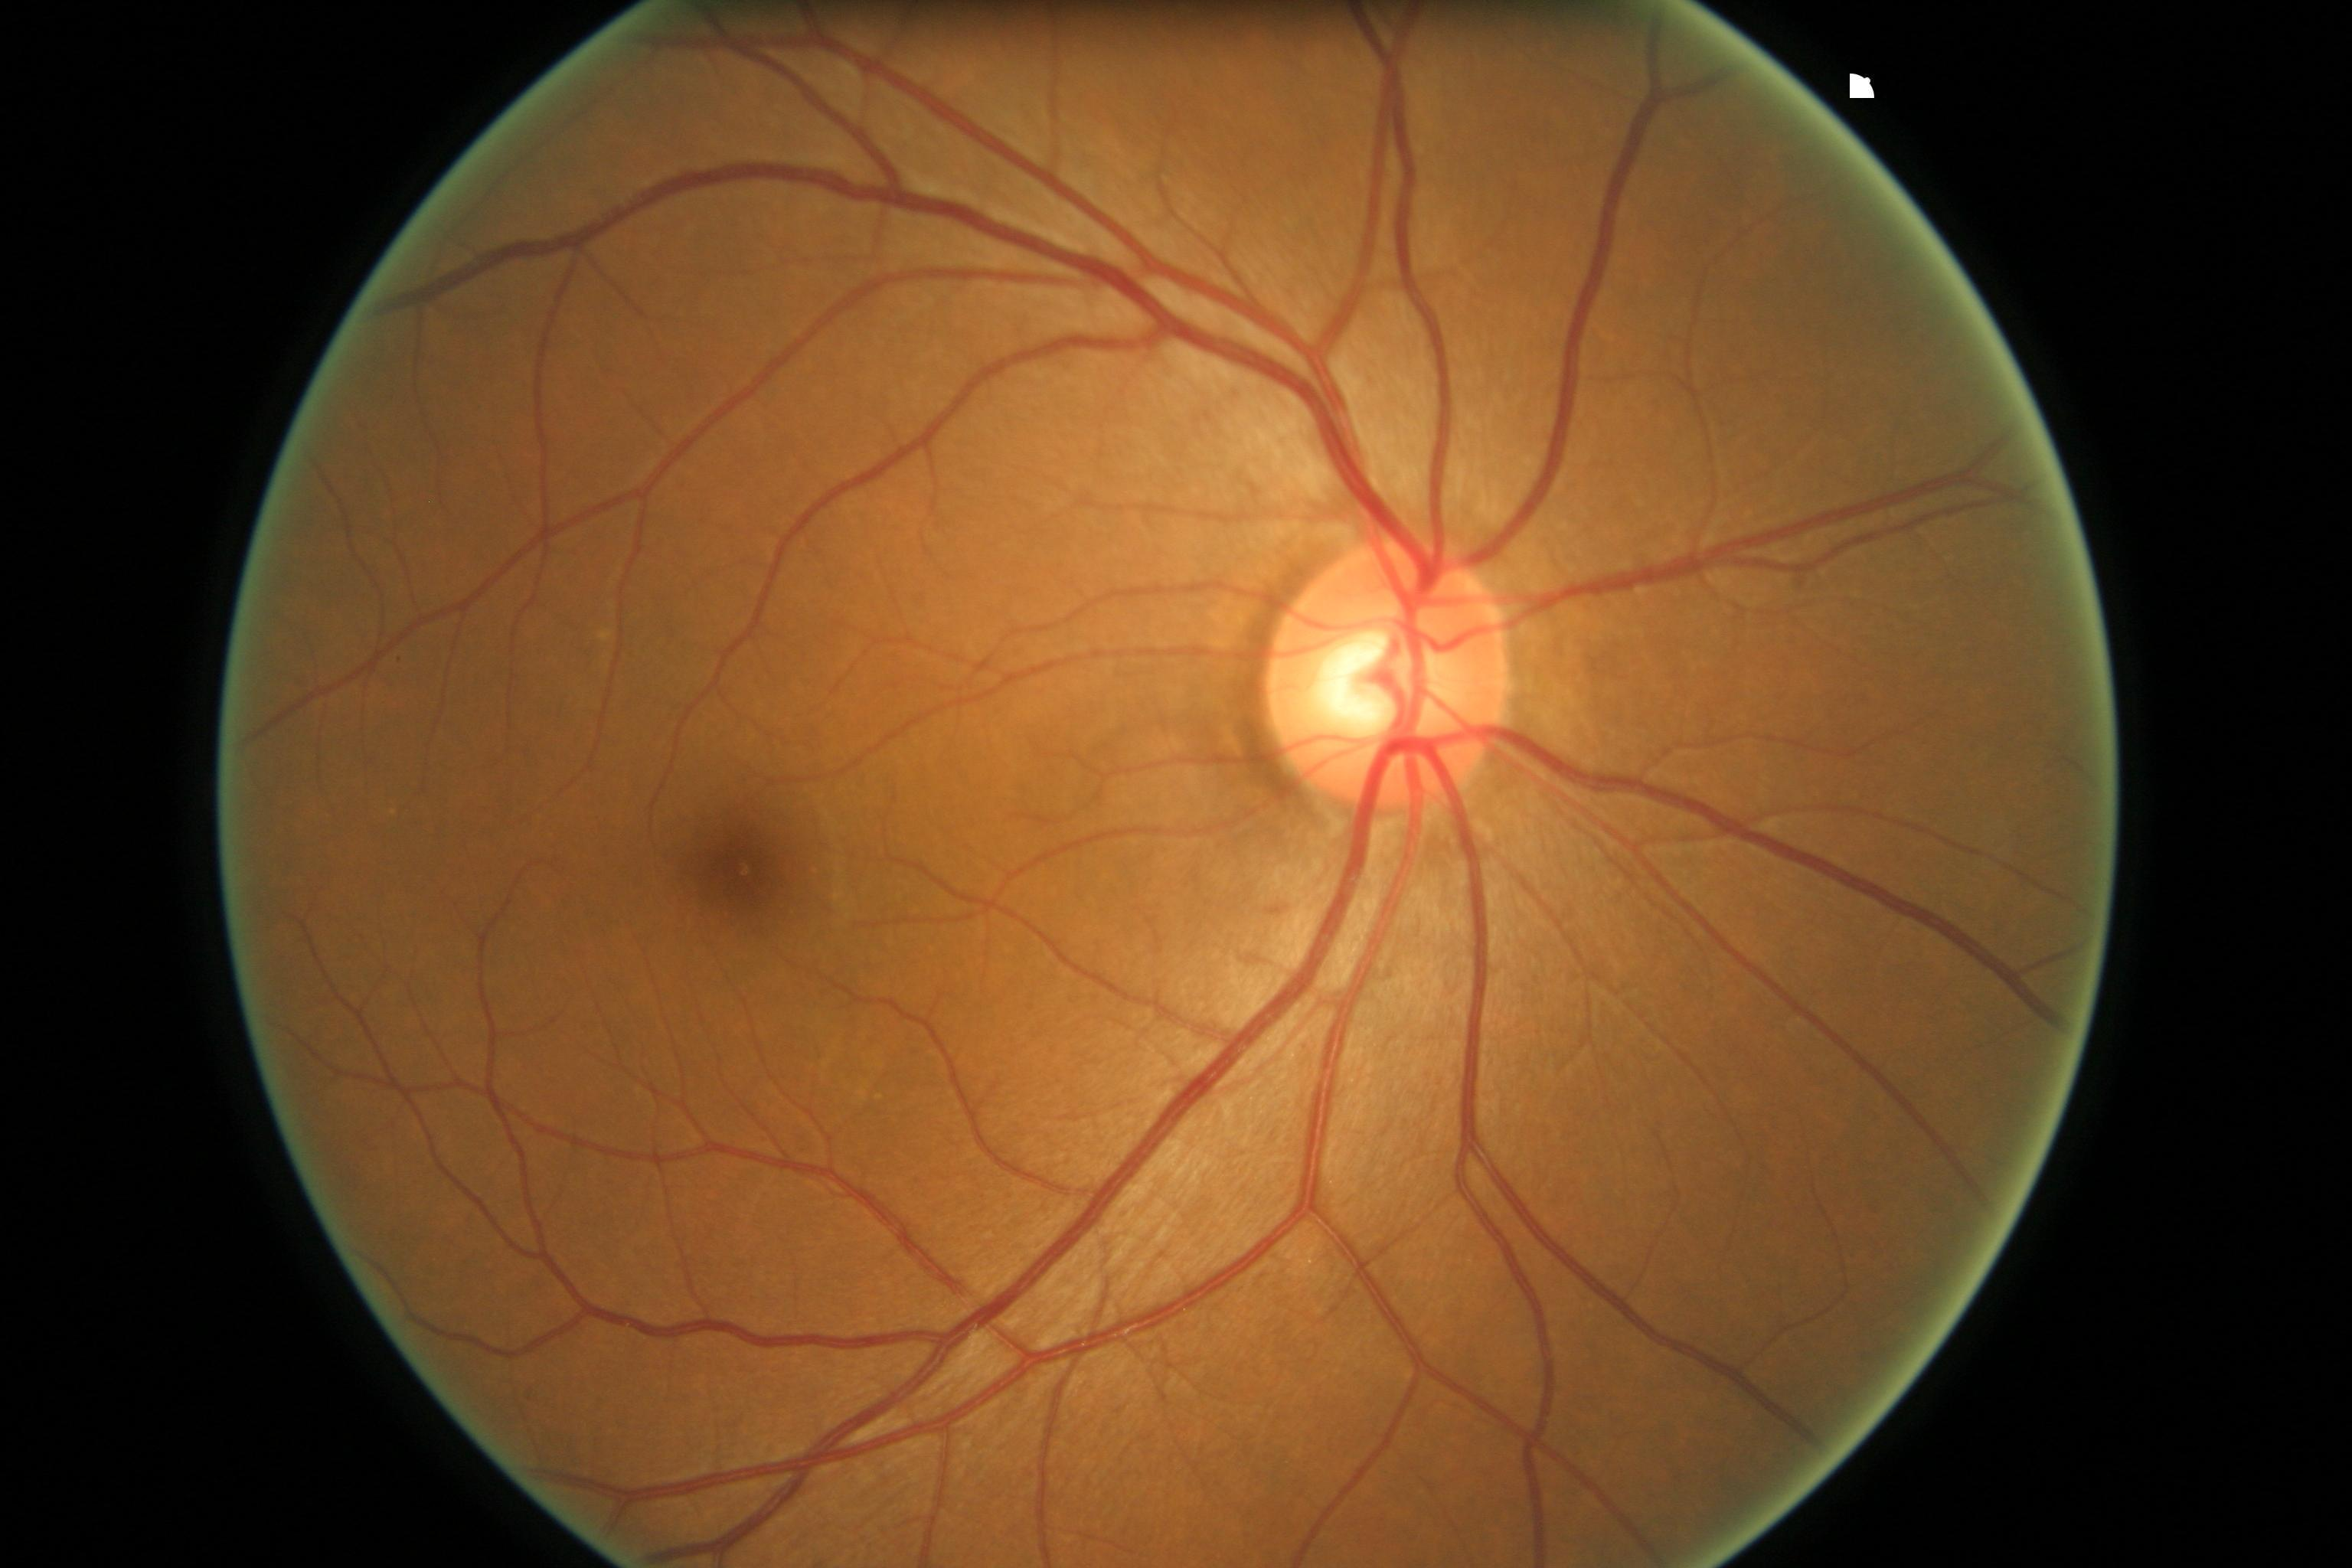
\includegraphics[width=7cm, height=6cm]{imgs/general/Retinal_fundus_image.jpg}
  \captionof{figure}{Retinal fundus image}
  \label{fig:Retinal_fundus_image}
\end{minipage}
\end{figure}
\noindent Here are some statistics and facts to appreciate the the relevance of this question:
\begin{itemize}
    \item People blind due to glaucoma: an estimated 4.5 million globally.
    \item Glaucoma is the second leading cause of blindness in the world after cataracts, but unlike cataracts, the vision loss associated with glaucoma is largely irreversible.
    \item Percentage of affected people who do not even know they have glaucoma: 
     \begin{itemize}
      \item Up to 50\% in developed countries.
      \item  It can go up to 90\% in underdeveloped parts of the world.
    \end{itemize}
    \item The size of the population with these eye diseases has increased by a factor of approximately 1.5 due to the increase in life expectancy of the population in the last 10 years.
    \item Once the retina is damaged, there is almost no chance of reversing vision loss unless some advances occur, such as stem cell therapy.
\end{itemize}
\subsection{Motivation}
There are two main motivations behind this project:
\begin{itemize}
    \item The possibility of helping to improve the quality of life of some people with something as important as having good vision.
    \item Learning more about computer vision, which is the field of machine learning that focuses on visual inputs such as images or videos, and how to develop a project in this field. This comes from motivation of wanting to develop projects of personal interest that make use of this type of data, such as medicine or art projects.
\end{itemize}
\subsection{Goals}
The goals for this project are:
\begin{itemize}
    \item Think of possible solutions that could help automate glaucoma detection with machine learning
    \item Explore different machine learning techniques to implement one or more of the solutions
    \item Implement and experiment with these techniques
    \item Analyze the experimentation results to see if this project provides viable solution to the glaucoma detection problem
    \item Analyze costs
\end{itemize}
\newpage\section{Problem analysis}
The first step in tackling the problem of glaucoma detection is to understand how experts do it, and then start thinking about possible ways to automate this process using retinal fundus imaging.
\subsection{How experts detect glaucoma}
Glaucoma is usually detected during a routine eye exam, often before it causes noticeable symptoms.  If the optometrist suspects that the patient has glaucoma after an eye test, there are different types of tests to confirm it and start treatment. These are eye pressure test, gonioscopy, visual field test and optic nerve assessment, the latter being the one that provides an image of the back of the eye, also known as a retinal fundus image. The issue here is that sometimes a single test is not enough to determine if the patient suffers from glaucoma, and other tests must be carried out to confirm it.
\\ 
\\ 
To detect glaucoma using retinal fundus images the experts use the cup-to-disc ratio (CDR). The CDR is a measurement used to assess the progression of glaucoma. See Figure \ref{fig:Example_of_vertical_cup_disc_ratio}.
\begin{figure}[H]
	\centering
	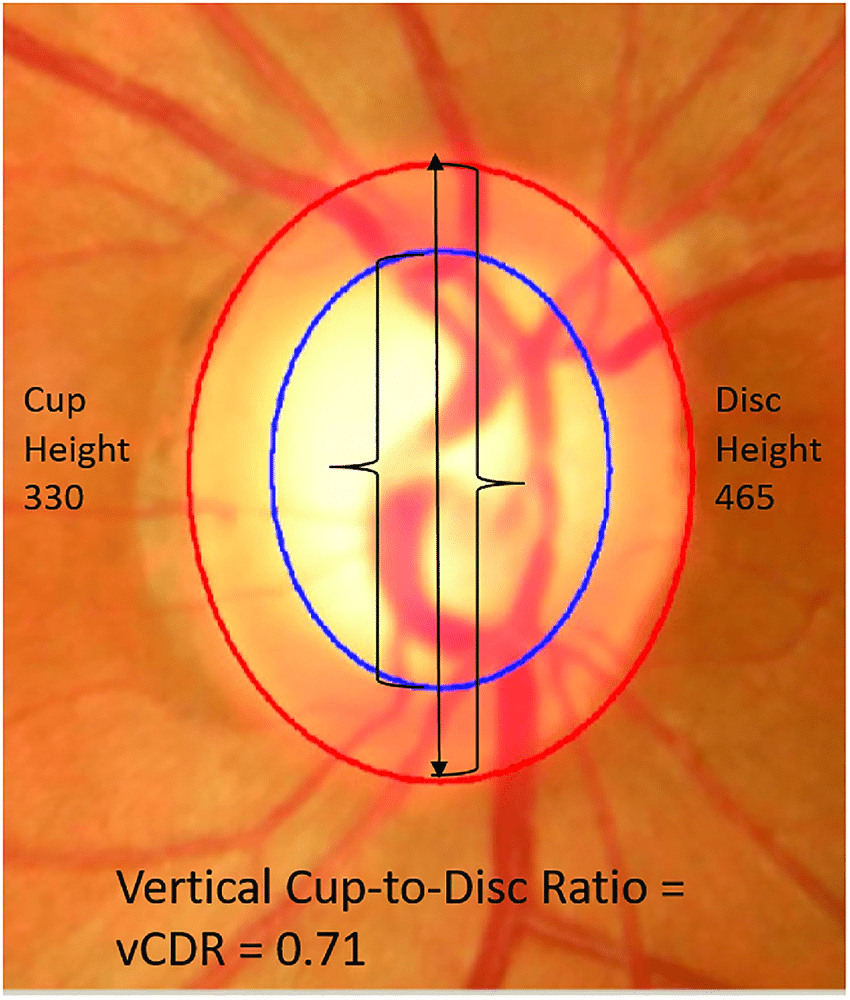
\includegraphics[width=8cm]{imgs/general/Example_of_vertical_cup_disc_ratio.png}
	\caption{Example of vertical cup disc ratio}
	 \label{fig:Example_of_vertical_cup_disc_ratio}
\end{figure}
\noindent The optic disc is the anatomical location of the eye's ``blind spot", the area where the optic nerve and blood vessels enter the retina. The optic disc can be flat or it can have a certain amount of normal cupping. But glaucoma, which is in most cases associated with an increase in intraocular pressure, often produces additional pathological cupping of the optic disc. The normal cup-to-disc ratio is 0.4. And a large cup-to-disc ratio may imply glaucoma or other pathology. See Figure \ref{fig:Optic_nerve_head_cupping_progression}. 
\begin{figure}[H]
	\centering
	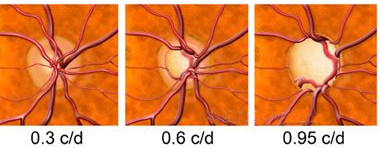
\includegraphics[width=12cm]{imgs/general/Optic_nerve_head_cupping_progression.jpg}
	\caption{Optic nerve head cupping progression}
	 \label{fig:Optic_nerve_head_cupping_progression}
\end{figure}
\noindent Other patterns that can denote glaucoma are optic nerves inflammation or movement. All of this is significant since the machine should identify these patterns in order to detect glaucoma. See Figure \ref{fig:Retinal_fundus_image} for a retinal fundus image of a healthy person and note that CDR is small. Then compare with Figure \ref{fig:2_examples_of_glaucoma_positive} of two positive cases of glaucoma where the CDR appears larger and the optic nerves seem to have moved.
\begin{figure}[H]
	\centering
	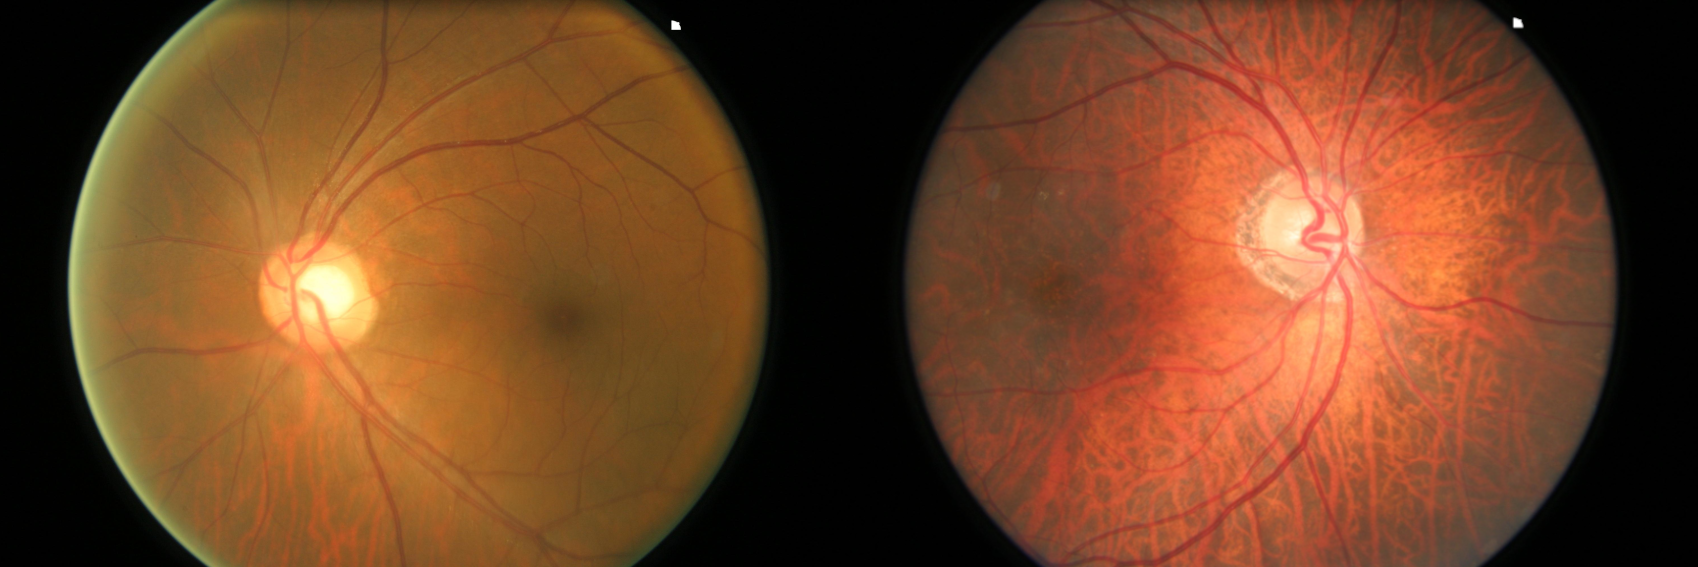
\includegraphics[width=15cm]{imgs/general/2_examples_of_glaucoma_positive.png}
	\caption{Two examples of glaucoma positive}
	 \label{fig:2_examples_of_glaucoma_positive}
\end{figure}

\subsection{How to automate glaucoma detection}
In machine learning, this problem falls under the category of binary classification. Binary because there is two categories ``Glaucoma positive" and ``Glaucoma negative" and classification because the goal is to classify new images into these two classes. This information will be useful to see how these kind of problems are usually solved. Additionally, this also provides an outline for project development, which is common to most machine learning projects. The general steps are:
\begin{enumerate}
  \item Collecting data
  \item Preparing the data
  \item Choosing a model, which will do the detection
  \item Training the model
  \item Evaluating the model
  \item Parameter tuning, to improve the model
  \item Comparing between different models
  \item Making predictions with the best model
\end{enumerate}
Knowing this, the perfect solution would be to make a machine learning model that could tell if a person has glaucoma or not. This is an approach that will be tested, but given that the implementation has to be highly reliable because its results affect people's health, and that previous work in this regard has shown the difficulty of obtaining this reliability, it will be worth exploring other approaches. Instead of making a model that is perfect at everything which would automate glaucoma detection 100\%, there is the option of making the model really good at just one thing, which reduces the resources needed to detect glaucoma.
\\
\\
Let's start by looking at the predictions about positive cases of glaucoma.
\\
First, let's look at the percentage of ``what the model predicted as glaucoma, which ones are glaucoma"". If 100\% accuracy were achieved in this area, it would mean that if the model says that a group of people are glaucoma positive, they are, but there may be some glaucoma positive cases that have not been detected. Could this information be useful in some way? Not so, because the doctor would have to test all the people who tested positive, but also the ones who tested negative, because there might be some cases there. For example, imagine a dataset with 100 cases, 50\% positive and 50\% negative. A model that predicted only 1 positive glaucoma and no negative glaucoma would get a score of 100\%, leaving 49 people with glaucoma unattended. This metric is called precision and will be explained in more detail in the ``Evaluation" section.
\\
However, if instead the focus is on trying to improve the percentage of people with glaucoma that the model detects as having glaucoma, this could yield valuable insights. Even if the model added false positives, this would save clinicians time and here's why. Imagine the dataset of the prior example, then a model that scores 100\% in this scenario could say that 75 people are glaucoma positive. This is not true as there is 50 glaucoma positive, but but due to the characteristics of the model, the 25 people detected as negative do not have glaucoma for sure. And the way this can be useful is that the resources optometrists save by not doing these 25 tests can be spent on testing more people. And to make sure this is a viable option, the worst case scenario in the last example would be that everyone is detected as glaucoma positive. In this case there would be no extra risk for the patients because they would all be cared for and there would be no saving of resources and everything would continue as it is now. Therefore, the worst case does not provide any improvement over the current situation, but all other possible scenarios avoid unnecessary testing. This metric is called recall, and will also delve into it later on.
\\
\\
Using the same logic for the negative cases, the bottom line is that they would not be useful or would lead to the same result.
\\
\\
In short, the idea is to develop a model that is excellent at either of these two tasks:
\begin{itemize}
    \item Detect who has glaucoma and who doesn't. This would make full automation possible in glaucoma detection.
    \item Detect everyone who has glaucoma, with the possibility of having false positives. This would avoid some unnecessary tests and save resources.
Both solutions would help prioritize more testing and treatment for positive glaucoma cases and could free up resources to help a larger population.
\end{itemize}
\section{Resources}
After analyzing the problem and finding two possible solutions to automate glaucoma detection, the available resources will define, to a certain extent, how to develop these solutions.
\subsection{Data}
After investigation, the data was obtained from ORIGA: An Online Retinal Fundus Image Database for Glaucoma Analysis and Research. This is currently the largest public dataset of glaucoma analyisis with retinal fundus images, and it consists of 650 images, including 168 glaucomatous images and 482 randomly selected nonglaucoma images. Each image is segmented and annotated by trained professionals from Singapore Eye Research Institute. The dataset is available at Kaggle\footnote{Kaggle Dataset:\url{https://www.kaggle.com/datasets/sshikamaru/glaucoma-detection}}. This is a fairly small dataset for image classification because the models tend to need a large amount of data to be accurate. However, there are techniques in both the preprocessing and modeling stages to deal with this.
\subsection{Development}
The development environment consists of Jupyter Notebook which provides different benefits that are useful when experimenting and evaluating models. Some of this are easy visualization and live code, which allows to break the code into parts so that a part of the code can be modified and executed without the need to re-execute the entire code again.
\\
\\
The chosen programming language is python because it has very complete high-level libraries and APIs that are widely used both for experimentation and for the implementation and deployment of models. Some of those used in the project are Scikit-learn, Keras, TensorFlow, Pandas, Numpy and Matplotlib. Although the models could be implemented from scratch, these libraries provide highly optimized implementations of the models and help save a lot of development time.
\subsection{Computing}
Training a model often takes a long time, so the better the hardware that runs the code, the faster the model will train. Because of their many cores, GPUs are often faster to train a model than CPUs, typically when more parallel computing is required. And there's even a faster processor unit designed specifically for AI, the TPU.
\subsubsection{Cloud}
This project started out as a Kaggle Notebook. However, due to the lack of flexibility in manipulating data on disk on this platform, it was changed to Google Colab. Colab offers plenty of RAM and powerful processing units that can be improved with a paid subscription. However, Colab has a drawback, it offers a limited execution time. So after a while of experimenting, it will ask to restart the whole run from 0, and if a model has a really long training time, it might not finish.
\\
\\
In this project Google Colab has been used to train and evaluate large models that were too time consuming to run locally.
\subsubsection{Local} 
Due to Colab's runtime limitation, most of the experimentation for this project has been done locally. The local advantages are unlimited runtime while the computer is on, and great flexibility in disk data manipulation, for example, reorganizing folders to try different data distributions.
\\
The computer specifications for this project have been:
\begin{itemize}
    \item 8GB of RAM
    \item Intel(R) Core(TM) i5-4430 CPU (3.00GHz)
    \item NVIDIA GeForce GT 630 GPU with 2GB of RAM
\end{itemize}
These are not powerful components, this is why some models took too long to run locally and were tested in the cloud. However, they served most of the experimentation without issue.

\section{Evaluation}
There are different ways to evaluate a model. In this project, the data has been separated into three sets, two to be used for training and one for testing. After training, the model will receive the images of the test set, which it has never seen before, and will classify each image in the test set as glaucoma positive or negative, based on what it learned from the other two sets. This classification will then be compared to the actual labels for each image. Some insights can then be extracted from this comparison to see how well the model generalizes to classify new data.
\\
\\
There are different metrics to determine how good a model is. During the following parts, the goal will be to improve the scores for these metrics, so choosing the right metrics is critical to developing a good solution.
Below are the most common metrics for binary classification and if they are valid for this project.
\subsection{Accuracy}
Accuracy is perhaps the simplest metric one can imagine and is defined as the ratio of correct predictions to the total number of predictions. In other words, what proportion of glaucoma predictions the model got right. However, this metric can sometimes be misleading because high accuracy does not always mean good results. Imagine a data set containing 100 images, 90 glaucoma negatives, and 10 glaucoma positives. A model that classifies all images in the dataset as negative for glaucoma would achieve an accuracy of 90\%, which is normally considered quite good. To make sure this is not the case, there are other metrics that explain the predictions in more depth, such as the confusion matrix.
\\
\\
How is this metric relevant to this project? Achieving an accuracy of 100\% would make the first proposed solution feasible and glaucoma detection could be fully automated, so it is a metric to take into account.
\subsection{Confusion Matrix}
A confusion matrix is a technique for summarizing the performance of a classification algorithm. Calculating a confusion matrix can give a better idea of what the classification model is getting right and what types of errors it is making. The number of correct and incorrect predictions is summarized with count values and broken down by each class. See figure \ref{fig:Confusion_matrix_for_binary_classification}.
\begin{figure}[H]
	\centering
	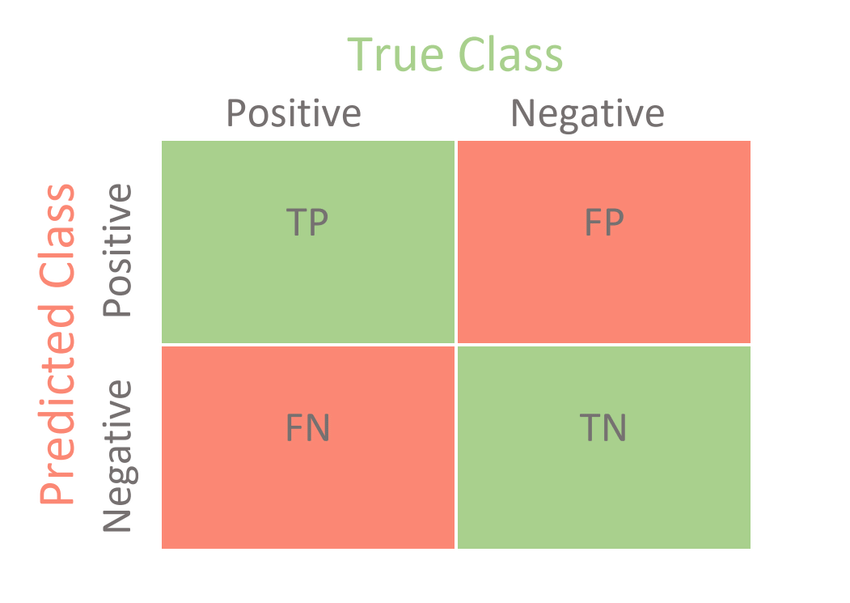
\includegraphics[width=10cm]{imgs/general/Confusion_matrix_for_binary_classification.png}
	\caption{Confusion matrix for binary classification}
	 \label{fig:Confusion_matrix_for_binary_classification}
\end{figure}
\noindent The labels in the squares have the following meaning for this project:
\begin{itemize}
    \item True Positives(TP): people with glaucoma that were correctly identified by the algorithm.
    \item True Negatives(TN): people without glaucoma that were correctly identified by the algorithm.
    \item False Negatives(FN): people who have glaucoma but the algorithm says they don't.
    \item False Positives(FP): people who do not have glaucoma but the algorithm says they do.
\end{itemize}
These variables are used to better understand the results and to calculate other metrics. See Figure \ref{fig:Results_CNN} for an example of a confusion matrix for this project.As can be seen, the cells of the matrix are colored so that the more cases that are represented in the cell, the more intense the color will be, with the result that it is possible to identify a model that accurately predicts for all classes by looking for a diagonal line of intensely colored cells from the top left to the bottom right (in other words, the cells where the predicted values match the actual values). 
\\
This is a good metric for this project because it gives a quick and accurate understanding of the overall performance of the model.
\subsection{Precision}
Precision explains how many of the correctly predicted cases actually turned out to be positive. Precision is useful in the cases where false positives are a higher concern than false negatives. The formula for calculating precision is:\\
TP / (TP+FP)
\\
As the definition says, precision focuses on the false positives and as stated in the problem analysis, there is no interest in improving only the precision. So this metric is not important for the project.
\subsection{Recall}
Recall explains how many of the actual positive cases the model is able to predict correctly. This is a useful metric in cases where false negatives are more of a concern than false positives. It is important in medical cases where it does not matter whether a false alarm is raised but the actual positive cases should not go undetected. This is precisely the case of the second proposed solution, so this metric will be taken into account. The formula for this is:\\
TP / (TP+FN)
\subsection{F1-Score}
F1-Score is an overall metric that essentially combines precision and recall. This is not relevant for the purposes of this project, so it will not be studied.
\subsection{ROC Curve and AUC}
The Receiver Operating Characteristic (ROC) curve is a plot that shows the performance of a binary classifier as a function of its cutoff threshold. Essentially, it shows the true positive rate (TPR) against the false positive rate (FPR) for various threshold values. Let's explain more.
Many of the classification models are probabilistic, i.e. they predict the probability of a sample being a cat. They then compare that output probability with some cut-off threshold and if it is larger than the threshold they predict its label as cat, otherwise as non-cat. As an example a model may predict the below probabilities for 4 sample images: [0.45, 0.6, 0.7, 0.3]. Then depending on the threshold values below, it will yield different labels:\\
cut-off= 0.5: predicted-labels= [0,1,1,0] (default threshold)\\
cut-off= 0.2: predicted-labels= [1,1,1,1]\\
cut-off= 0.8: predicted-labels= [0,0,0,0]\\
By varying the threshold values, the results are completely different labels. And as the predictions may be modified for each of these scenarios, it would result in a different precision and recall (as well as TPR, FPR) rates. To clarify, TPR and recall are the same thing and FPR is the the proportion of incorrect predictions in positive class. The ROC curve essentially finds out the TPR and FPR for various threshold values and plots the TPR against the FPR. A sample ROC curve is shown in Figure \ref{fig:Sample_ROC_curve}.
\begin{figure}[H]
	\centering
	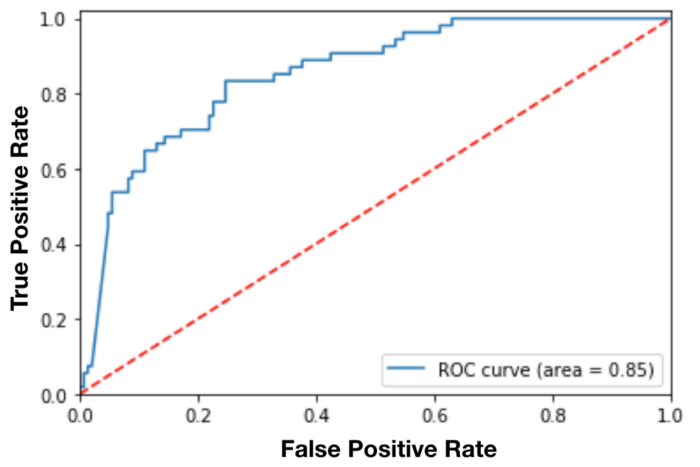
\includegraphics[width=10cm]{imgs/general/Sample_ROC_curve.png}
	\caption{Example of a ROC curve}
	 \label{fig:Sample_ROC_curve}
\end{figure}
The larger the area under the curve (which can be any value from 0 to 1), the better the model is performing - this is the AUC metric. To get an idea of how this area represents model performance, see the straight diagonal line from the bottom left to the top right of the ROC chart. This represents the expected performance if
each patient diagnosis was decided by guessing or flipping a coin, because about half of the predictions would be correct. So the area under the diagonal line represents an AUC of 0.5. If the AUC for a model is higher than this for a binary classification model, then the model performs better than a random guess.
\\\\ For this project, the ROC curve can be useful to pick a good cut-off threshold and the AUC to get a general idea of how the model is performing.

\section{Models}
A machine learning model is a file that has been trained to recognize certain types of patterns. A model is trained over a set of data, providing it an algorithm that it can use to reason over and learn from those data. Once the model is trained, it can reason over data that it hasn't seen before, and make predictions about those data. In this section there is an explanation of the chosen models, which will be evaluated later in the Results section.
\\\\
All the implementations made for this project can be found in this Github repository \footnote{Github repository: \url{https://github.com/notaiax/Glaucoma-Detection-ML}}. 
\subsection{Convolutional Neural Network}
A convolutional neural network (CNN) or convnet is a model capable of extracting features from images and finding patterns to make predictions. This is exactly what the experts do to detect glaucoma. So, since the CNN is good at finding patterns and extracting knowledge from them, it might be good at finding which cup-to-disc ratio combined with which nerve inflammation or movement is a possible case of glaucoma. However, to make sure, let's see a general idea of how a convnet works.\\\\
\begin{figure}[H]
	\centering
	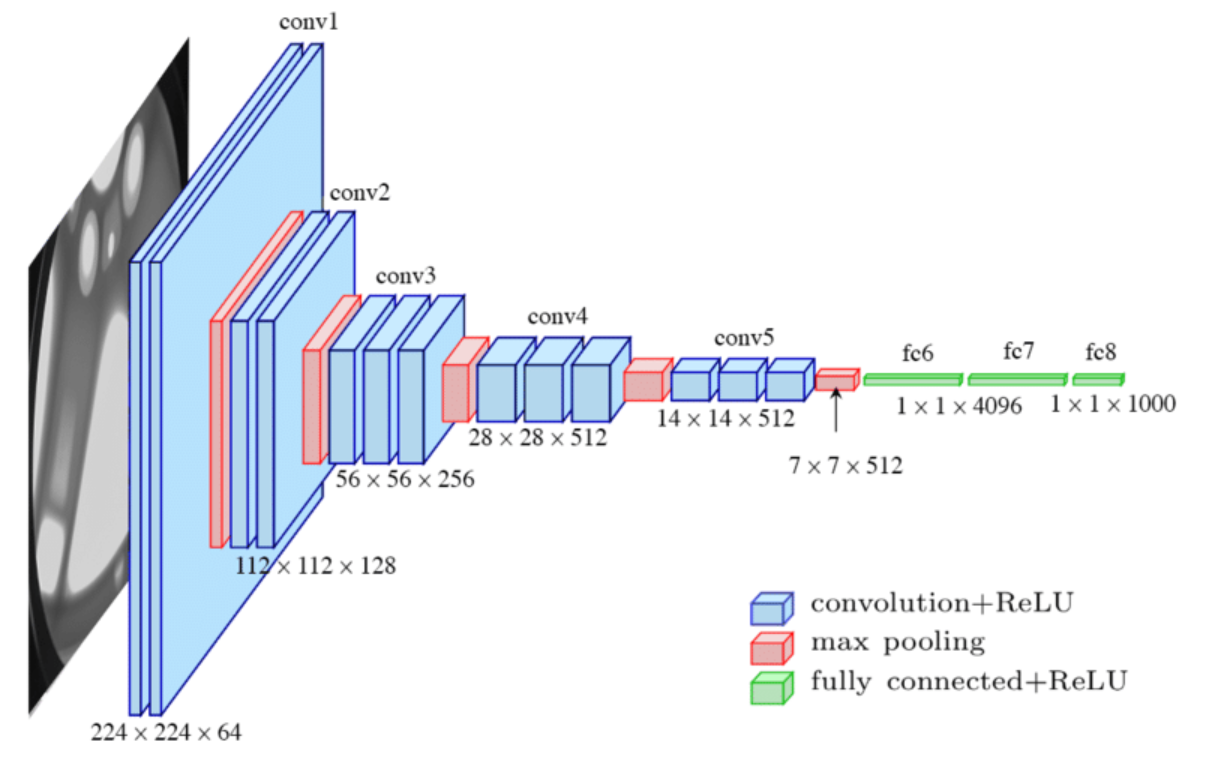
\includegraphics[width=12.5cm]{imgs/general/VGG16-CNN-Architecture.png}
	\caption{VGG16 CNN Architecture}
	 \label{fig:VGG16-CNN-Architecture}
\end{figure}
\noindent A CNN is a neural network made up of multiple layers, which can be separated into two groups for this type of model:
\begin{itemize}
    \item Base: The base is used to extract the features from an image. It is made up of three different types of layers that are represented in Figure \ref{fig:VGG16-CNN-Architecture} in red and blue. These are:
    \begin{itemize}
        \item Convolution: A convolutional layer carries out the filtering step. In short, a convolution is a function that scans an image to find patterns like lines, circles, edges, etc. In the CDR case, the convolutional layers would detect two circles, the optical disc and the optical cup.
        \item ReLU: After filtering, the feature maps pass through the activation function that performs the detection step, by keeping only the data of the image filtered by the convolution. Continuing with the CDR example, the ReLU layers would remove everything from the image except the two detected circles.
        \item Maximum Pooling: Notice that after applying the ReLU function (Detect) the feature map ends up with a lot of "dead space," that is, large areas containing only 0's (the black areas in the image). Having to carry these 0 activations through the entire network would increase the size of the model without adding much useful information. Instead, it would better to condense the feature map to retain only the most useful part -- the feature itself. This in fact is what maximum pooling does. Max pooling takes a patch of activations in the original feature map and replaces them with the maximum activation in that patch. So in the case of the CDR, the MaxPool layers would accentuate the circles and reduce the image size.
    \end{itemize}
    \item Head: The head is used to determine the class of the image using the features that the base extracted. It is mainly made up of dense layers, but might include other layers such as dropout. These are the green layers in Figure \ref{fig:VGG16-CNN-Architecture}. Wrapping up the CDR example, the head would receive information about the two detected circles, look for a pattern, and perhaps discover that a larger CDR is a common feature among positive glaucoma cases.
\end{itemize}
This looks like a promising model. Nonetheless, these models tend to need larger datasets than the current 650 images in this project dataset. So let's look at a tool that could help with this.
\subsection{Transfer Learning}
Transfer learning is a valuable tool in deep learning that allows individuals to access the knowledge learned from very complex models trained on millions of labeled images. Running these models can take weeks, even when multiple GPUs are used, making it not feasible for the average individual to build. These are known as pretrained models.
\\\\
The intuition behind transfer learning for image classification is that if a model is trained on a large and general enough dataset, this model will effectively serve as a generic model of the visual world. Therfore, it is possible to take advantage of these learned feature maps without having to start from scratch by training a large model on a large dataset. This could be useful because in this project, because if a CNN is not able to extract enough features from the ORIGA dataset, features from previous images could make up for it.
\\\\
The problem here is that these models are usually trained in everyday things like a jackfruit or a syringe. So they probably didn't see a single retinal fundus image during training, let alone try to detect glaucoma from it. As a curiosity, during the experimentation a retinal fundus image was passed to the model and it was predicted to be an orange, due to the similarity in shape and color. So the first step in transferring the learning is that the model predicts only between positive and negative glaucoma. This is done with feature extraction.

\subsubsection{Feature Extraction}
Feature extraction consists of using the representations learned by a previous network to extract meaningful features from new samples. By simply adding a new classifier or head, which will be trained from scratch, on top of the pretrained model, it can reuse previously learned feature maps.
\paragraph{VGG16}\mbox{}\\
VGG16 is a famous CNN architecture considered as an excellent vision model architecture. See Figure \ref{fig:VGG16-CNN-Architecture}. To perform feature extraction on this model, the fully connected layers are replaced with a custom classifier. There is one type of average pool that is widely used at the head of a convnet.
This is the global average pool. A GlobalAvgPool2D layer is often used as an alternative to some 
or all of the hidden Dense layers in the head of the network, like in the implementation on Github. GlobalAvgPool2D simply replaces the entire feature map with its average value. Though very destructive, it often works quite well and has the advantage of reducing the number of parameters in the model.
\paragraph{ResNet-50}\mbox{}\\
Like VGG16, ResNet-50 is a CNN architecture that is well known for its good performance, with the difference that it is considerably larger. While VGG16 has 16 layers, ResNet-50 has 50 layers, as the names indicate. The steps to perform feature extraction are the same as for VGG16, and this will also be evaluated to see if the difference in model size affects the results.
\subsubsection{Fine-Tuning}
The layers of the pretrained model are frozen, so when the model is retrained to transfer learning, its knowledge is not lost. However, sometimes the feature extraction will not work well because the feature extraction part is not good enough on the new data. This is where fine tuning comes into play. It consists of unfreezing some upper layers of the frozen pretrained model base and training both the newly added classifier layers and the last layers of the base model together. This allows to "fine-tune" the higher-order feature representations in the base model in order to make them more relevant for the specific task.
\paragraph{VGG16}\mbox{}\\
For this part, the procedure is the same as in the feature extraction model, but the base block5 has been unfrozen. This means unfreezing from layer 15. More details about the layers are available in the implementation.
\paragraph{ResNet-50}\mbox{}\\
For this part, the procedure is the same as in the feature extraction model, but the base conv5 blocks has been unfrozen. This means unfreezing from layer 143. More details about the layers are available in the implementation.

\subsection{Hyperparameters}
In machine learning, a hyperparameter is a parameter whose value is used to control the learning process. By contrast, the values of other parameters (typically node weights) are derived via training. One cannot know the exact best value for hyperparameters for the given problem. The best value can be determined either by the rule-of-thumb or by trial and error. 
\\\\
After looking up the rule-of-thumb hyperparameters and tuning them, here are the final hyperparameters for the models that gave the best results
\begin{itemize}
    \item Optimizer: Adam with learning\_rate=0.0001
    \item Early stopping with a patience=5, min\_delta=0.001 and restore\_best\_weights=True
    \item Batch size: 10
    \item Epochs: 20
\end{itemize}
The chosen loss function is binary\_crossentropy because it is intended for use with binary classification where the target values are in the set \{0, 1\}. 

\section{Data Preparation}
Before training the model, it is necessary to prepare the data.
\subsection{Distribution}
In order to create and evaluate the model, the original dataset has been splited into three sets.
\begin{itemize}
    \item Training set: Contains the data used to train the model.
    \item Validation set: It is used for frequent evaluation to fine-tune the model hyperparameters. Therefore, the model occasionally sees this data, but never learns from it. However, by adjusting the hyperparameters in response to the results of evaluating these data, the validation set indirectly affects the model.
    \item Test set: This set it is used to evaluate the model once the model has been completely trained and provides an unbiased evaluation.
\end{itemize}
After some tests, the ORIGA dataset has been splitted with a distribution of 40\% for the training set, 40\% for the validation set and 20\% for the test set. 

\subsection{Preprocessing}
Data preprocessing is the act of modifying the input dataset to make it more suitable for training and testing. An important step in preprocessing is data cleaning, which involves removing duplicates, dealing with outliers, and so on. However, since the dataset has been created and reviewed by professionals, this step has been skipped.

\subsubsection{Data Augmentation and Balancing}
The ORIGA datasets presents two potential problems. The first is that there may not be enough data to train an accurate model. The second one is that the data is unbalanced. 74\% of the dataset are glaucoma negative cases and only 26\% are glaucoma positive. The problem here is that if the model detects that as a pattern, it could tend to classify more images as negative for glaucoma. Both these problems can be solved with data augmentation.
\\\\
Data augmentation is a technique used to increase the amount of data by adding slightly modified copies of already existing data or newly created synthetic data from existing data. There are different ways to augment the data such as image rotation, resizing, moving the image (x pixels), etc. For this project it has been studied that the ways to augment the data should be the horizontal flip and the color contrast. See Figure \ref{fig:Retinal fundus image with its augmentations}. Another advantage of using data augmentation is better generalization.
\begin{figure}[H]
	\centering
	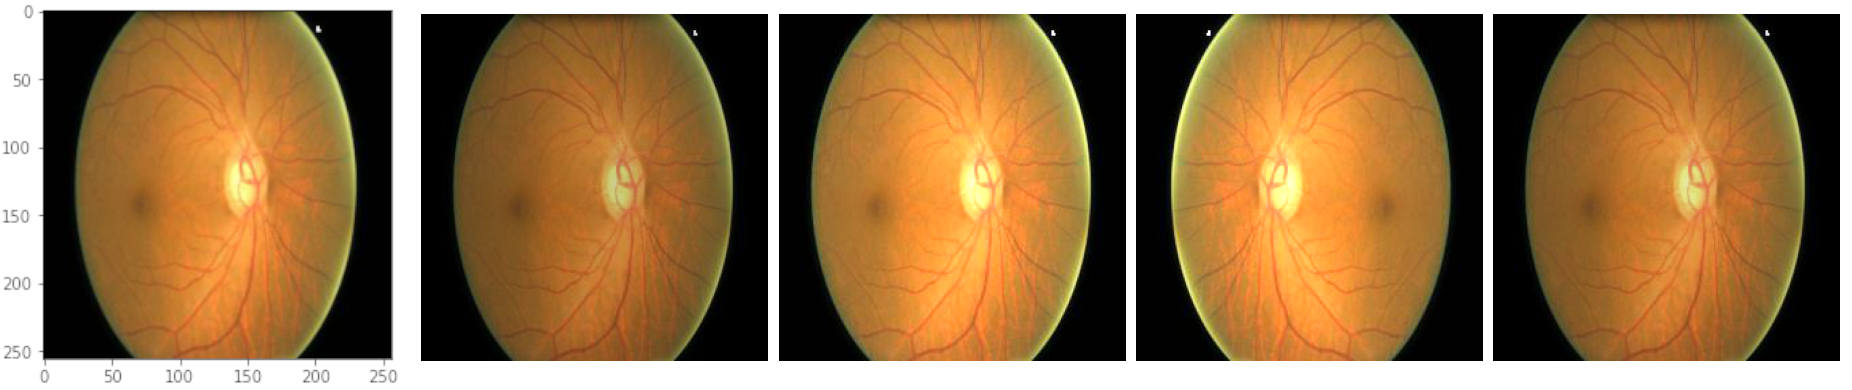
\includegraphics[width=15cm]{imgs/general/Retinal fundus image with its augmentations.png}
	\caption{Retinal fundus image with data augmentation (horizontal flip and color contrast)}
	 \label{fig:Retinal fundus image with its augmentations}
\end{figure}
\noindent The data has been balanced on the training set, because that is what the model uses to learn from and there should be no bias there. To balance the data, the less common cases (Glaucoma Positive), have been augmented until there was the same cases that Glaucoma positive. See Figure \ref{fig:Data distribution before data balancing} and \ref{fig:Data distribution after data balancing}.
\begin{figure}[H]
\centering
\begin{minipage}{.5\textwidth}
  \centering
  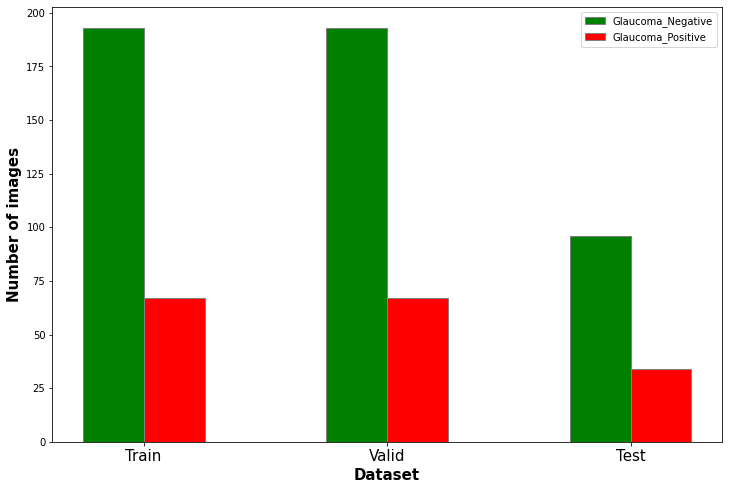
\includegraphics[width=7cm, height=6cm]{imgs/general/Data distribution before data balancing.png}
  \captionof{figure}{Initial data distribution}
  \label{fig:Data distribution before data balancing}
\end{minipage}%
\begin{minipage}{.5\textwidth}
  \centering
  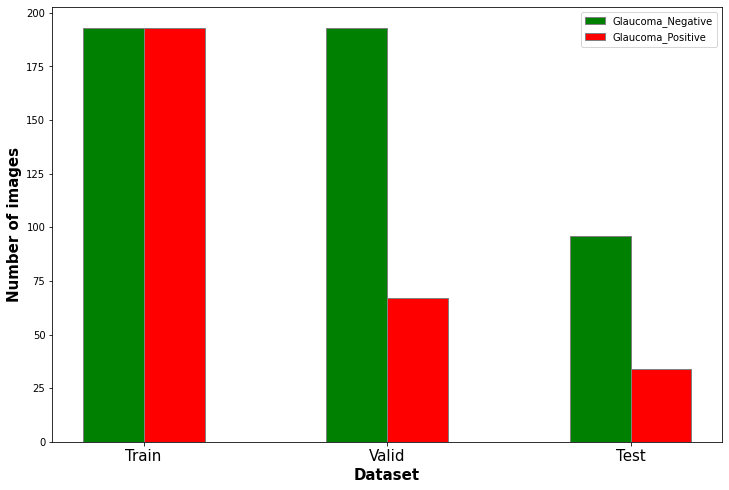
\includegraphics[width=7cm, height=6cm]{imgs/general/Data distribution after data balancing.png} 
  \captionof{figure}{Data distribution after balancing}
  \label{fig:Data distribution after data balancing}
\end{minipage}
\end{figure}
\noindent The data augmentation to increase the dataset size has been added as preprocessing layers in the model.

\subsubsection{Dimensionality Reduction}
When defining the model architecture, one of the requisites is to define a fixed input shape. When performing this task, it is important to keep in mind that there is a balance between computation speed and information loss. To elaborate, when the size of an image is reduced, information is removed (pixels). Less information means faster training times and less memory usage; however, it also may mean reduced overall accuracy. To be compatible with the pretrained models used for transfer learning, an image size of 224 x 224 was selected. See Figure \ref{fig:Batch of images with no preprocessing}. 
\begin{figure}[H]
	\centering
	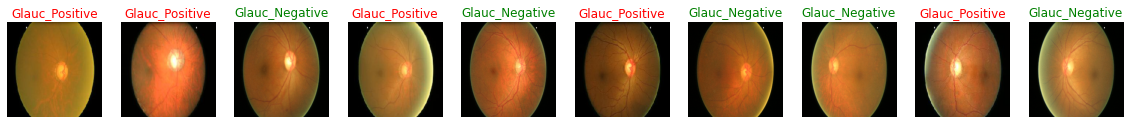
\includegraphics[width=15cm]{imgs/general/Batch of images with no preprocessing.png}
	\caption{Batch of redimensioned images}
	 \label{fig:Batch of images with no preprocessing}
\end{figure}
\subsubsection{VGG16 Preprocessing}
VGG16 preprocessing is used to preprocess data for the model architecture VGG16. However, after testing it with a custom CNN architecture, it returned better results than just using dimensionality reduction. In addition, the best model of all those developed in this project was trained using data treated by this preprocessor. When using VGG16 preprocessor, images are converted from RGB to BGR, then each color channel is zero-centered with respect to the ImageNet dataset, without scaling. See Figure \ref{fig:Batch of images preprocessed with VGG16}. 
\begin{figure}[H]
	\centering
	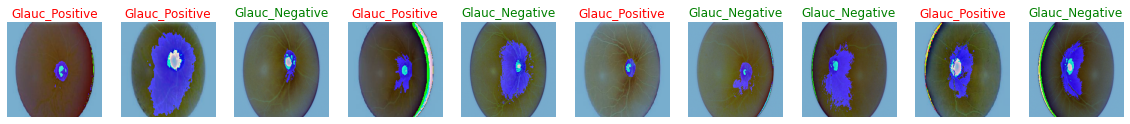
\includegraphics[width=15cm]{imgs/general/Batch of images preprocessed with VGG16.png}
	\caption{Batch of images preprocessed with VGG16}
	 \label{fig:Batch of images preprocessed with VGG16}
\end{figure}


\section{Results}
None of the models achieved 100\% accuracy or recall, so none of the following models would be valid for the presented solutions. However, the results are interesting to see how the different models perform in this task.

\subsection{Convolutional Neural Network}
Surprisingly, after trying many different architectures and hyperparameter settings, the convnet that gave the best result was the smallest and simplest one:
\begin{verbatim}
Sequential([
    Conv2D(filters=32, kernel_size=(3, 3), activation='relu', padding = 'same', 
    input_shape=(224,224,3)),
    MaxPool2D(pool_size=(2, 2), strides=2),
    Conv2D(filters=64, kernel_size=(3, 3), activation='relu', padding = 'same'),
    MaxPool2D(pool_size=(2, 2), strides=2),
    Flatten(),
    Dense(units=2, activation='softmax')
])
\end{verbatim}
See Figure \ref{fig:Results_CNN}. Accuracy is 70\%, recall 44\%, and looking at the ROC curve there is no threshold to help achieve 100\% recall, apart from predicting everything as positive glaucoma which has no utility. The AUC shows that the model is better than just randomly guessing who has glaucoma because 0.634$>$0.500. However, this is not a valid solution for this project.
\begin{figure}[H]
	\centering
	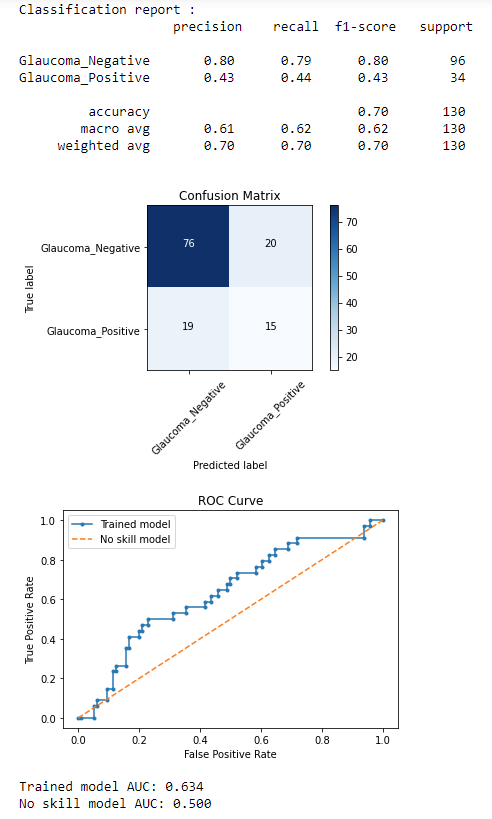
\includegraphics[width=12cm]{imgs/results/Results_CNN.png}
	\caption{CNN evaluation results}
	 \label{fig:Results_CNN}
\end{figure}
\subsection{Transfer Learning}
Contrary to expectations, the evaluation of these models is not much higher than that of CNN.
\subsubsection{Feature Extraction}
Feature extraction yielded the best results for this project.
\paragraph{VGG16}\mbox{}\\
See Figure \ref{fig:results-vgg16-fe}. Accuracy is 69\%, recall 50\%, and looking at the ROC curve there is no threshold that helps to achieve 100\% recall. Although the CNN accuracy it was higher, it can be determined by the recall and AUC that this model performs better, being the one with the best evaluation for this project.
However, this is not a valid solution for this project because it does not meet accuracy or recall standards.

\paragraph{ResNet-50}\mbox{}\\
See Figure \ref{fig:results-resnet50-fe}. The results are similar to those of VGG16 with the difference that the recall is much lower. This can probably be modified by adjusting the threshold, so the take away is that the base pretrained model did not make a remarkable difference, at least with VGG16 and ResNet-50.
\begin{figure}[H]
\centering
\begin{minipage}{.5\textwidth}
  \centering
  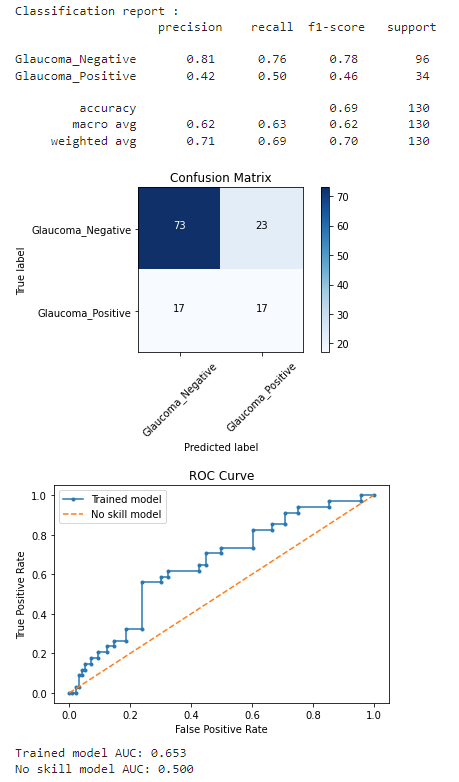
\includegraphics[width=8cm, height=15cm]{imgs/results/results-vgg16-fe.PNG}
  \captionof{figure}{Evaluation results of VGG16\\ with feature extraction}
  \label{fig:results-vgg16-fe}
\end{minipage}%
\begin{minipage}{.5\textwidth}
  \centering
  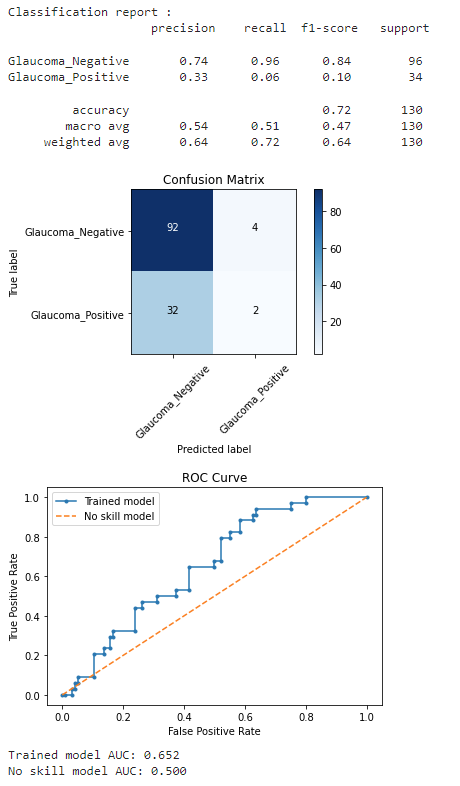
\includegraphics[width=8cm, height=15cm]{imgs/results/results-resnet50-fe.PNG} 
  \captionof{figure}{Evaluation results of ResNet-50 with feature extraction}
  \label{fig:results-resnet50-fe}
\end{minipage}
\end{figure}
\subsubsection{Fine-Tuning}
See Figure \ref{fig:results-vgg16-ft} and \ref{fig:results-resnet50-ft}. Note that both models obtained the same classification report with little differences in the ROC curve. These two models obtained the highest accuracy among the different models, yet the performance is the worst when looking at the other metrics. For example, in both models, the positive glaucoma recall is 0\% and an AUC is 55\%. Considering that the AUC gives a general idea of the model's performance, these models are only slightly better than a model that would take random guesses to make predictions. All this happens because the models are classifying everything as positive glaucoma. Since this is the predominant class in the test set, it gives good accuracy but poor recall and AUC.
\begin{figure}[H]
\centering
\begin{minipage}{.5\textwidth}
  \centering
  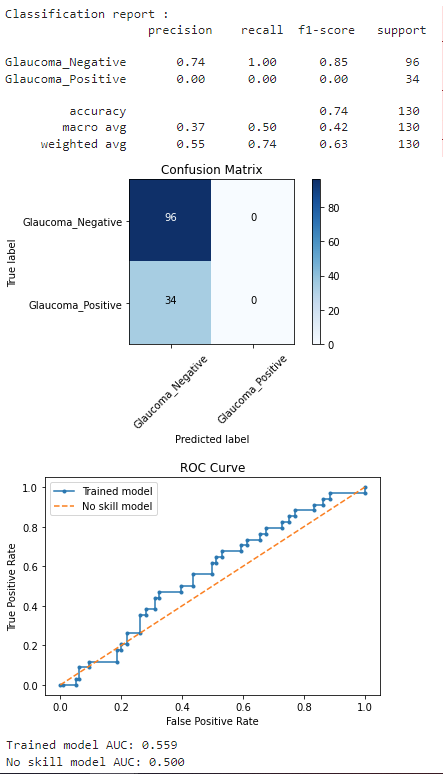
\includegraphics[width=8cm, height=15cm]{imgs/results/results-vgg16-ft.PNG}
  \captionof{figure}{Evaluation results of VGG16\\ with fine-tuning}
  \label{fig:results-vgg16-ft}
\end{minipage}%
\begin{minipage}{.5\textwidth}
  \centering
  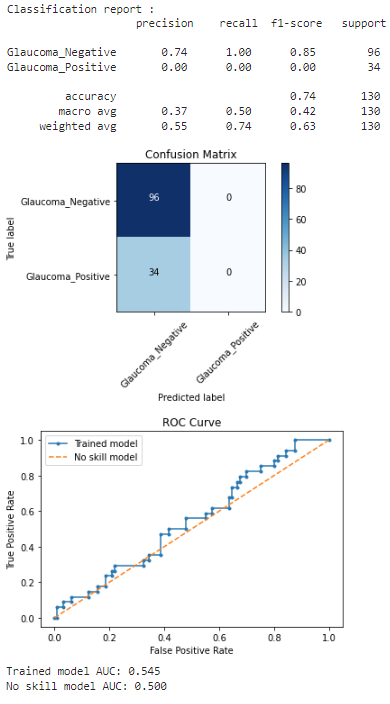
\includegraphics[width=8cm, height=15cm]{imgs/results/results-resnet50-ft.PNG} 
  \captionof{figure}{Evaluation results of ResNet-50 with fine-tuning}
  \label{fig:results-resnet50-ft}
\end{minipage}
\end{figure}

\section{Costs}
See table \ref{tab:Costs and results table}. The training costs of these models are not high compared to other models that can take hours or days to train. As seen in the table, all the models but the CNN have been trained with a GPU. This is because while the CNN has only a few layers, the other models are built with more layers, that are more complex and time consuming than the CNN ones. GPU offers better parallellization than CPU when it comes to model training, leading to faster training times. To see this difference in numbers, training the VGG16 Feature Extraction model took 34:17 minutes on CPU, nearly three times that on GPU. And while this training time seems like nothing compared to what some other models require, doing hyperparameter tuning requires performing this training multiple times, which adds up and is quite time consuming. All the GPU models have been trained using Google Colab with the free plan, and the CNN model has been trained in local with an Intel(R) Core(TM) i5-4430 CPU (3.00GHz).
\begin{table}[H]
\begin{tabular}{|c|c|c|c|c|c|c|}
\hline
\rowcolor[HTML]{C0C0C0} 
\textbf{Model}                                                             & \cellcolor[HTML]{C0C0C0}\textbf{\begin{tabular}[c]{@{}c@{}}Training \\ Time \\ (MM:SS)\end{tabular}} & \cellcolor[HTML]{C0C0C0}\textbf{\begin{tabular}[c]{@{}c@{}}Processing \\ Unit\end{tabular}} & \textbf{Accuracy} & \textbf{Recall} & \textbf{AUC} & \textbf{Conclusions}                                                                                                                    \\ \hline
\begin{tabular}[c]{@{}c@{}}VGG16 \\ Feature \\ Extraction\end{tabular}     & 12:24                                                                                                & GPU                                                                                         & 69\%              & 50\%            & 65.3\%       & \cellcolor[HTML]{9AFF99}\begin{tabular}[c]{@{}c@{}}Best model \\ but inviable\end{tabular}                                              \\ \hline
CNN                                                                        & 04:55                                                                                                & CPU                                                                                         & 70\%              & 44\%            & 63.4\%       & \cellcolor[HTML]{FFFC9E}\begin{tabular}[c]{@{}c@{}}Not a bad score \\ but inviable\end{tabular}                                         \\ \hline
\begin{tabular}[c]{@{}c@{}}ResNet-50 \\ Feature \\ Extraction\end{tabular} & 11:46                                                                                                & GPU                                                                                         & 72\%              & 6\%             & 65.2\%       & \cellcolor[HTML]{FFFC9E}\begin{tabular}[c]{@{}c@{}}Not a bad score \\ but inviable\end{tabular}                                         \\ \hline
\begin{tabular}[c]{@{}c@{}}VGG16 \\ Fine-Tuning\end{tabular}               & 12:39                                                                                                & GPU                                                                                         & 74\%              & 0\%             & 55.9\%       & \cellcolor[HTML]{FFCCC9}\begin{tabular}[c]{@{}c@{}}Inviable. The\\  model classifies \\ everything as\\  glaucoma positive\end{tabular} \\ \hline
\begin{tabular}[c]{@{}c@{}}ResNet-50 \\ Fine-Tuning\end{tabular}           & 12:34                                                                                                & GPU                                                                                         & 74\%              & 0\%             & 54.5\%       & \cellcolor[HTML]{FFCCC9}\begin{tabular}[c]{@{}c@{}}Inviable. The\\  model classifies \\ everything as\\  glaucoma positive\end{tabular} \\ \hline
\end{tabular}
\caption{\label{tab:Costs and results table} Costs and results}
\end{table}

\section{Predictions Explainability}
Model evaluation gives insight into how the model is performing, however it is often unclear how the neural network arrives at these conclusions. In fact, these algorithms where the user cannot see the inner workings of the algorithm are called black box algorithms
\begin{figure}[H]
	\centering
	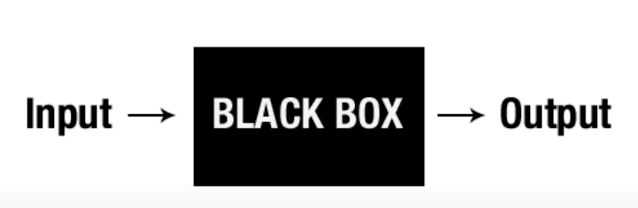
\includegraphics[width=12cm]{imgs/general/Black box algorithm.PNG}
	\caption{Black box algorithm}
	 \label{fig:Black box algorithm}
\end{figure}
\noindent Fortunately, tools exist to understand what's going on inside a model and determine if the model can be trusted. Let's see why understanding this is so important with an example. See Figure \ref{fig:Husky-Wolf classifier predictions} to see the predictions made by a model that classifies between wolves and huskies. 
\begin{figure}[H]
	\centering
	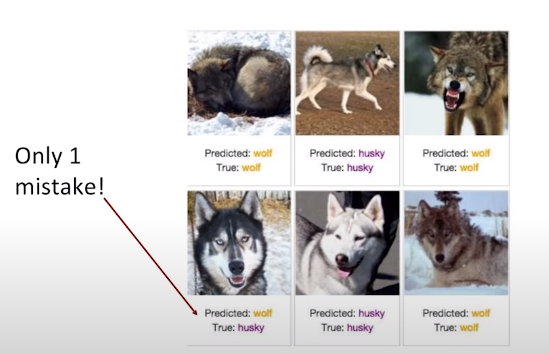
\includegraphics[width=14cm]{imgs/general/Husky-Wolf classifier predictions.PNG}
	\caption{Husky-Wolf classifier predictions}
	 \label{fig:Husky-Wolf classifier predictions}
\end{figure}
\noindent At first glance this looks like a good model that only made one mistake. However, see Figure \ref{fig:Husky-Wolf classifier predictions explanation}  to see what the model used to make the predictions. The image on the left shows the original image and the one on the right shows which part of the original image made the model make its prediction. See that the model detects wolves by looking if there is snow on the image. This gives good performance because wolves happen to appear in snowy landscapes and huskies don't. So, even though this predictions would perform really well on the evaluation metrics seen so far, is this a good model? It's a great snow detector, but it's not a good wolf and husky classifier because then the focus would have been on parts of the wolf, like its face, instead of the snow.
\begin{figure}[H]
	\centering
	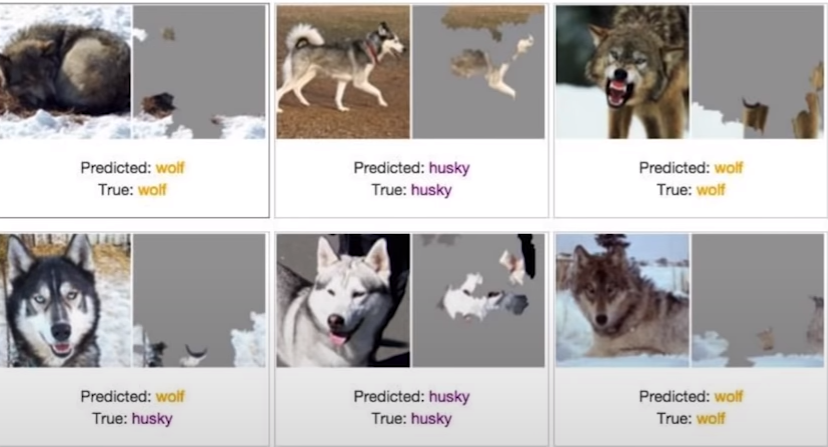
\includegraphics[width=14cm]{imgs/general/Husky-Wolf classifier predictions explanation.PNG}
	\caption{Husky-Wolf classifier predictions explanation}
	 \label{fig:Husky-Wolf classifier predictions explanation}
\end{figure}
\noindent Therefore, being able to interpret the output of the models can be useful for many things. First, to see why a model is not performing well, by seeing what the model interprets as useful information. Second, if the model works well, the explanation tools can help identify problems like the one in the wolf example. Finally, if the explanations of the prediction make sense, it gives the developer and the client the assurance that the model is reliable. And in a medical case like glaucoma detection, in addition to assuring the doctor that the model is focusing on the right points, it could help find useful new patterns that weren't detected before.

\subsection{Predictions Explanation with Lime}
Lime is a tool to explain what machine learning classifiers (or models) are doing. Lime is short for local interpretable model-agnostic explanations, which means that it can explain individual predictions for any model, be it a neural network, random forest, or other. Additionally, it supports images and tabular data (numpy arrays of numeric or categorical data). See Figure \ref{fig:Lime explaining prediction of 'Cat' in pros and cons}.
\begin{figure}[H]
	\centering
	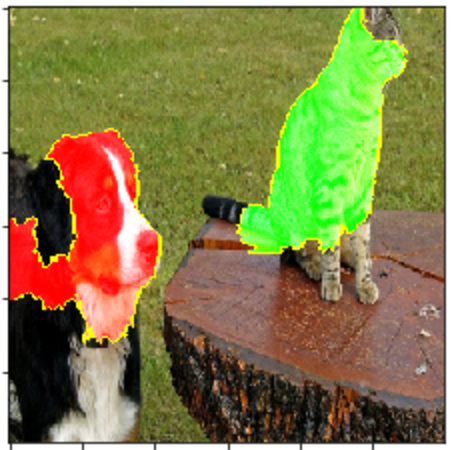
\includegraphics[width=8cm]{imgs/general/Lime explaining prediction of 'Cat' in pros and cons.png}
	\caption{Lime explaining prediction of 'Cat' in pros and cons}
	 \label{fig:Lime explaining prediction of 'Cat' in pros and cons}
\end{figure}
\noindent  After analyzing a batch of image predictions made with the best model of this project (VGG16 with transfer learning), these have been the results:
\begin{figure}[H]
	\centering
	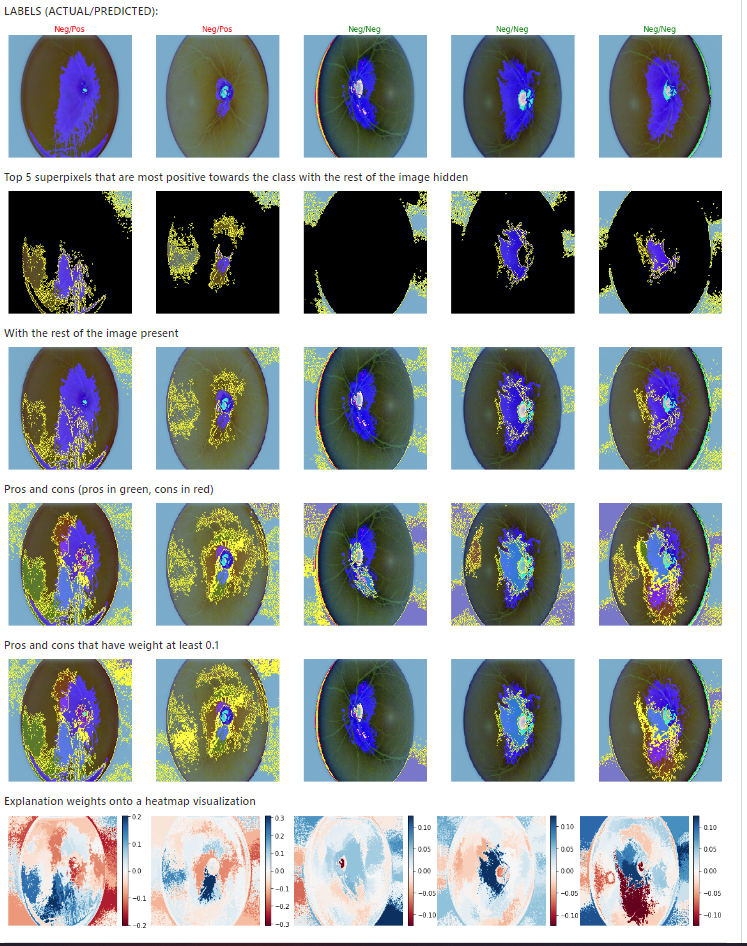
\includegraphics[width=15cm]{imgs/general/Glaucoma detection predictions explained with Lime.PNG}
	\caption{Glaucoma detection predictions explained with Lime}
	 \label{fig:Glaucoma detection predictions explained with Lime}
\end{figure}
\noindent It can be seen that the model does not really focus on relevant parts like the cup disc, optic disc, or optic nerves. So, as inferred from the evaluation results and confirmed with lime, this model cannot be trusted. All other models have reached similar results.


\section{Future work}
These are possible ways to improve the results that could not be tested and have been left as future work:
\begin{itemize}
     \item Implement and test a model using the MONAI framework for image classification. This is a framework focused on healthcare images and uses PyTorch and DenseNet for the classification.
     \item Use the ACRIMA dataset. The images in this dataset focus on the center of the eye, which contains the information needed to calculate the CDR and appreciate the movement of the optic nerve. This dataset can be found on the same Kaggle page where the ORIGA dataset was obtained.
     \item Test the attention technique so that the model focuses on specific things like the CDR or the optic nerves.
     \item Try different heads like XGBoost for the best model (VGG16 with feature extraction).
    \item Explore more advanced machine learning techniques.
\end{itemize}


\section{Conclusions}
In the analysis of the problem, it has been concluded that to automate glaucoma, a model with an accuracy or recall of almost 100\% would be necessary. Then, it has been found that different CNN architectures, combined with techniques such as transfer learning, balanced data augmentation, vgg16 preprocessing, and hyperparameter tuning, do not solve the problem. Although the evaluation showed acceptable results with some of the models, being the best in the VGG16 model with feature extraction, it did not meet the standards to become a real solution. Furthermore, when the predictions made by this model were interpreted with lime, it was found that the model did not focus on the most important parts of the image. 
\\\\ After all, the conclusion is that to solve the glaucoma detection problem with machine learning it is not enough with these models and the ORIGA dataset. However, exploring other datasets like ACRIMA with other more specialized models like the MONAI 2d classification could lead to better results. To explore possible improvements, it is recommended to reuse the project implementation available on GitHub. This comes with all the necessary implementations for data visualization, pre-processing or model evaluation, leaving only the task of adding new models or techniques. This project can also be mostly reused for other image binary classification projects.
\\\\
Regarding the costs, training this type of model can take up to 15 minutes in environments such as Google Colab. This isn't much, but when experimenting and tuning hyperparameters, it can be time consuming.
\\\\ Personally, this project has been useful for me to learn how to develop an computer vision project with good practices. Examples of this would be having a deeper understanding of what the model is actually doing using lime or having a deep understanding of the different evaluation techniques and not relying on accuracy alone. These are techniques that once learned are easy to implement and that I will undoubtedly extrapolate to future projects.
\newpage
\begin{thebibliography}{9}
\bibitem{}
Robert N. Weinreb, Tin Aung, Felipe A. Medeiros. \emph{The Pathophysiology and Treatment of Glaucoma. \url{https://www.ncbi.nlm.nih.gov/pmc/articles/PMC4523637/}}. 2014
\bibitem{}
Rupert R. A. Bourne, Hugh R. Taylor, Seth R. Flaxman, Jill Keeffe, Janet Leasher, Kovin Naidoo, Konrad Pesudovs, Richard A. White, Tien Y. Wong, Serge Resnikoff, Jost B. Jonas, Vision Loss Expert Group of the Global Burden of Disease Study. \emph{Number of People Blind or Visually Impaired by Glaucoma Worldwide and in World Regions 1990 – 2010: A Meta-Analysis. \url{https://www.ncbi.nlm.nih.gov/pmc/articles/PMC5072735/}}. 2016
\bibitem{}
Aurélien Geron. \emph{Hands-on Machine Learning with Scikit-Learn, Keras, and TensorFlow: Concepts, Tools, and Techniques to Build Intelligent Systems. Second edition}. 2019
\bibitem{}
Keiron O'Shea, Ryan Nash. \emph{An Introduction to Convolutional Neural Networks
. \url{https://arxiv.org/abs/1511.08458?context=cs}}. 2015
\bibitem{}
Karen Simonyan, Andrew Zisserman. \emph{Very Deep Convolutional Networks for Large-Scale Image Recognition. \url{https://arxiv.org/abs/1409.1556}}. 2015
\bibitem{}
Kaiming He, Xiangyu Zhang, Shaoqing Ren, Jian Sun. \emph{Deep Residual Learning for Image Recognition. \url{https://arxiv.org/abs/1512.03385?context=cs}}. 2015
\bibitem{}
Zhuo Zhang, Fengshou Yin, Jiang Liu, Wing Kee Wong,
Ngan Meng Tan, Beng Hai Lee, Jun Cheng, Tien Yin Wong . \emph{ORIGA-light : An Online Retinal Fundus Image Database for Glaucoma Analysis and Research. \url{https://oar.a-star.edu.sg/storage/n/n2od11j13o/embc10-zhangz-apr12-v2.pdf}}. 
\bibitem{}
Karimollah Hajian-Tilaki. \emph{Receiver Operating Characteristic (ROC) Curve Analysis for Medical Diagnostic Test Evaluation. \url{https://www.ncbi.nlm.nih.gov/pmc/articles/PMC3755824/}}. 2013
\bibitem{}
Fuzhen Zhuang, Zhiyuan Qi, Keyu Duan, Dongbo Xi, Yongchun Zhu, Hengshu Zhu, Senior Member, IEEE,
Hui Xiong, Fellow, IEEE, and Qing He. \emph{A Comprehensive Survey on Transfer Learning. \url{https://arxiv.org/pdf/1911.02685.pdf}}. 2020 
\bibitem{}
Muhammad Naseer Bajwa, Muhammad Imran Malik, Shoaib Ahmed Siddiqui, Andreas Dengel, Faisal Shafait, Wolfgang Neumeier, Sheraz Ahmed. \emph{Two-stage framework for optic disc localization and glaucoma classification in retinal fundus images using deep learning. \url{https://www.ncbi.nlm.nih.gov/pmc/articles/PMC6637616/}}. 2019
\bibitem{}
Marco Tulio Ribeiro, Sameer Singh, Carlos Guestrin. \emph{"Why Should I Trust You?": Explaining the Predictions of Any Classifier.\url{https://dl.acm.org/doi/10.1145/2939672.2939778}}. 2016
\bibitem{}
Andres Diaz-Pinto, Sachidanand Alle, Alvin Ihsani, Muhammad Asad, Vishwesh Nath, Fernando Pérez-García, Pritesh Mehta, Wenqi Li, Holger R. Roth, Tom Vercauteren, Daguang Xu, Prerna Dogra, Sebastien Ourselin, Andrew Feng, M. Jorge Cardoso. \emph{MONAI Label: A framework for AI-assisted Interactive Labeling of 3D Medical Images. \url{https://arxiv.org/abs/2203.12362}}. 2022
\bibitem{}
Ashish Vaswani, Noam Shazeer, Niki Parmar, Jakob Uszkoreit, Llion Jones, Aidan N. Gomez, Lukasz Kaiser, Illia Polosukhin. \emph{Attention Is All You Need. \url{https://arxiv.org/abs/1706.03762}}. 2017

\end{thebibliography}
\end{document}
